\documentclass[russian,english]{llncs}
\usepackage[utf8]{inputenc}
\usepackage[T2A]{fontenc}
\usepackage[final]{graphicx}
\usepackage{epstopdf}
\usepackage[labelsep=period]{caption}
\usepackage[hyphens]{url}
\usepackage{amssymb,amsmath,mathrsfs}
\usepackage[russian,english]{babel}
%\usepackage{multicol}
\usepackage[ruled,vlined,linesnumbered,algo2e]{algorithm2e}
%\usepackage{algorithm}
%\usepackage[noend]{algorithmic}
\usepackage{color}
\usepackage{cmap}
\usepackage{array}
\usepackage{tikz}
\usepackage{pgfplots}
%\usepackage{verbatim}
\usepackage{standalone}

\tolerance=1000
\hbadness=5000
\newcommand{\const}{\mathrm{const}}
\newcommand{\tsum}{\mathop{\textstyle\sum}\limits}
\newcommand{\tprod}{\mathop{\textstyle\prod}\limits}
\newcommand{\cov}{\mathop{\rm cov}\limits}
\newcommand{\Dir}{\mathop{\rm Dir}\nolimits}
\newcommand{\norm}{\mathop{\rm norm}\limits}
\newcommand{\KL}{\mathop{\rm KL}\nolimits}
%\renewcommand{\geq}{\geqslant}
%\renewcommand{\leq}{\leqslant}
\newcommand{\eps}{\varepsilon}
\newcommand{\cond}{\mspace{3mu}{|}\mspace{3mu}}
\newcommand{\Loss}{\mathscr{L}}
\newcommand{\RR}{\mathbb{R}}
\newcommand{\cL}{\mathscr{L}}
\newcommand{\cP}{\mathscr{P}}
\newcommand{\kw}[1]{\textsf{#1}}
\SetKwFor{ForAll}{\textbf{for all}}{}{}

%... and these rows too.
\pgfplotsset{ every non boxed x axis/.append style={x axis line style=-},
     every non boxed y axis/.append style={y axis line style=-}}
\pgfplotsset{compat = 1.3}

\begin{document}
%%Analysis of Images, Social Networks, and Texts
\title{
    Parallel Non-blocking Deterministic Algorithm for Online Topic Modelling
}
\author{
    Oleksandr Frei\inst{1}
    \and
    Murat Apishev\inst{2}
}
\institute{\noindent
    Schlumberger Information Solutions,
    ~~\email{oleksandr.frei@gmail.com}
    \and
    Lomonosov Moscow State University,
    ~~\email{great-mel@yandex.ru}
}

\maketitle

\begin{abstract}
In this paper we present a new algorithm for inference of additively regularized topic models
and discuss key architectural details of our implementation.
The key property of the new algorithm is that it behaves in a fully deterministic fashion,
which is typically hard to achieve in a non-blocking parallel implementation.
The algorithm had been recently implemented in the BigARTM library (\texttt{http://bigartm.org}),
and in our experiments it performs better comparing to the previous versions in term of convergence,
CPU utilization and memory usage.

\vspace{1em}
\textbf{Keywords:}
    probabilistic topic modeling,
    Probabilistic Latent Sematic Analysis,
    Latent Dirichlet Allocation,
    Additive Regularization of Topic Models,
    stochastic matrix factorization,
    EM-algorithm,
    BigARTM.
\end{abstract}

\section{Introduction}

Deterministic behavior is an important property for any algorithm,
including those of a stochastic nature.
For the end users of a software system run-to-run reproducibility is a must-have property,
because this is what they expect based on their previous experience.
Indeed, refreshing a web-pages or re-doing an operation in almost any software
produce the same result as before, regardless of how much complexity is hidden behind the scenes.
For the researches determinism is also important
because it enables them to reproduce their old experiments
and study impact of various parameters on the result.
Finally, for the developers of the algorithm
determinism allow to write simple unit-tests with well-defined results.

Determinism is particularly hard to achieve
in concurrent implementations, because in a multi-threaded environment
it might not be sufficient to just fix a random seed or an initial approximation.
In this paper we present a deterministic modification of parallel non-blocking algorithm
for online topic modeling, previously developed for BigARTM library.
We implement new algorithm in BigARTM and demonstrate that new version converges faster
than previous algorithm in terms of perplexity,
yet being more efficient in CPU and memory usage.

The rest of the paper is organized as follows.
In~section~\ref{sec:Previous}
we introduce basic notation and summarize previous algorithm for online topic modeling, used in $BigARTM v0.6$.
In~section~\ref{sec:Algorithm}
we~present a deterministic non-blocking modification of the algorithm.
In~section~\ref{sec:Architecture}
we~describe the architecture, implemented in $BigARTM v0.7$.
In~section~\ref{sec:Experiments}
we~report results of our experiments on large datasets.
In~section~\ref{sec:Conclusions}
we~discuss advantages, limitations and open problems of BigARTM.

%sashafrey:
%really technical topics in my opinion does not belong to AISTconf article;
%it would be more appropriate to discuss the following in the full 12-page article in http://www.ispras.ru/en/ journal
%\begin{itemize}
%    \item Details of CLI interface and python interface, usage examples
%    \item List new features: coherence score and regularizer, classification, documents markdown (aka $p_{tdw}$ matrices)
%    \item Our technologies (Protobuf for low-level C API, Boost Serialize for import/export, GLog, GFlags, GTest, etc)
%    \item Our build solution and CI solution (CMake, Visual Studio, GitHub, Git submodules, Travis, Apveyour, Read-The-Docs)
%    \item Why people care about run-to-run reproducibility
%    https://software.intel.com/en-us/articles/consistency-of-floating-point-results-using-the-intel-compiler
%\end{itemize}

\section{Previous algorithm}
\label{sec:Previous}

\SetAlgoSkip{}
\begin{algorithm2e}[t]
\caption{Offline algorithm}
\label{alg:Offline}
\BlankLine
\KwIn{collection $D$;}
\KwOut{matrix $\Phi = (\phi_{wt})$;}
\BlankLine
initialize $(\phi_{wt})$\;
\Repeat{$(\phi_{wt})$ converges}{
    %$\tilde n_{wt} := 0$ for all $w \in W$ and $t \in T$\;
    %\ForAll{documents $d \in D$} {
    %    $(\tilde n_{wt}) := (\tilde n_{wt}) + \kw{ProcessDocument}(d, \Phi)$\;
    %}
    $(n_{wt}) := \mathlarger\sum\limits_{d \in D} \; \kw{ProcessDocument}(d, \Phi)$\;
    $(r_{wt}) := \dots \text{ (calc regularization)}$\;
    $(\phi_{wt}) := \norm_{w \in W} (\tilde n_{wt} + r_{wt})$\;
}
\end{algorithm2e}
\begin{algorithm2e}[t]
\caption{\kw{ProcessDocument}($d, \Phi$)}
\label{alg:ProcessDocument}
\BlankLine
\KwIn{document $d \in D$, matrix $\Phi=(\phi_{wt})$;}
\KwOut{matrix $(\tilde n_{wt})$;}
\BlankLine
initialize $\theta_{td} := \frac{1}{|T|}$ for all $t \in T$\;
\Repeat{$\theta_d$ converges}{
    $p_{tdw} := \norm_{t\in T} \bigl(\phi_{wt}\theta_{td}\bigr)$ for all $w\in d$ and $t \in T$\;
    $n_{td} := \sum_{w\in d} n_{dw} p_{tdw}$ for all $t \in T$\;
    $r_{td} := \dots \text{ (calc regularization)}$\;
    $\theta_{td} := \norm_{t\in T}
        \bigl(
            n_{td} + r_{td}
        \bigr)$ for all $t \in T$\;
}
$\tilde n_{wt} := n_{dw} p_{tdw}$ for all $w \in d$ and $t \in T$\;
\end{algorithm2e}

Let
$D$ denote a finite set (collection) of texts and
$W$ denote a~finite set (vocabulary) of all terms from these texts.
Let
$n_{dw}$ denote the number of occurrences of a term $w \in W$ in a document $d \in D$;
$n_{dw}$ values form a sparse matrix $N_{dw}$ of size $|W| \times |D|$,
known as \emph{bag-of-words} representation of the collection.

Given an $N_{dw}$ matrix, an additively-regularized topic model infers two stochastic matrices:
$\Phi = \{\phi_{wt}\}$ and $\Theta = \{\theta_{td}\}$,
of sizes $|W| \times |T|$ and $|T| \times |D|$ respectively,
where $|T|$ is a used-defined number of \emph{topics} in the model.
Matrices $\Phi$ and $\Theta$
provide a compressed representation of the $N_{dw}$ matrix:
\[
n_{dw} \approx n_d \sum_{t \in T} \phi_{wt} \theta_{td}, \text { for all } d \in D, w \in W,
\]
where $n_d = \sum_{w \in W} n_{dw}$ denotes the total number of terms in a document $d$.

Inference of $\Phi$ and $\Theta$ can be done via Offline EM-Algorithm
(see Algorithm \ref{alg:Offline} and \ref{alg:ProcessDocument}).
Key step of the algorithm is $\kw{ProcessDocument}$ subroutine
that generates a matrix $\hat n_{wt}$ of size $n_d \times |T|$.
These values describe contribution of the tokens from the document into the final $\Phi$ matrix.
Then the offline algorithm aggregates $\hat n_{wt}$ values across all documents in the collection.
After normalization they form a new $\Phi$ matrix for the next iteration.
Note that $\theta_{td}$ values appear only within $\kw{ProcessDocument}$ subroutine.
This makes the algorithm efficient in its memory usage,
allowing implementation to not store the entire theta matrix.
Instead, $\theta_{td}$ values are recalculated from scratch on every pass through the collection.

To improve convergence rate of the algorithm 
the collection can be split into ``batches''.
The algorithm is adjusted so that
matrix $\Phi$
is re-calculated after each batch, incorporating information about new documents.
Key difference is that the cumulative sum $n_{wt}$ is discounted by a factor $\rho_b < 1$,
which depends on the iteration. Typical strategy is to use $\rho_b = \dots$.

The new $\Phi$ matrix is based on a weighted sum of the previous $n_{wt}$ matrix
and new $\hat n_{wt}$ values produced for the latest batch.
This leads to the Online algorithm \ref{alg:Online}.

% ToDo: define ``norm'' operator somewhere...
%``norm'' operator transforms
%a~real vector $(x_i)$ to
%a~vector $(x'_i)$ representing a discrete distribution:
%\[
%    x'_i = \norm(x_i) = \frac{\max\{x_i,0\}}{\sum_{j} \max\{x_j,0\}}.
%\]

%A drawback of the algorithm \ref{alg:Offline} is that the entire collection is processed with a single $\Phi$ matrix.

\SetAlgoSkip{}
\begin{algorithm2e}[h]
\caption{Online algorithm} %\mbox{regularized} topic modeling
\label{alg:Online}
\BlankLine
\KwIn{collection $D$;}
\KwOut{matrix $\Phi = (\phi_{wt})$;}
\BlankLine
form batches $D := D_1 \sqcup D_2 \sqcup \dots \sqcup D_B$\;
initialize $(\phi^0_{wt})$\;
\ForAll{batches $D_b$, $b = 1,\dots,B$} {
    $(\hat n_{wt}) := \mathlarger\sum\limits_{d \in D_b} \; \kw{ProcessDocument}(d, \Phi)$\;
    $(n^b_{wt}) := \rho_b \cdot (n^{b-1}_{wt}) + (1 - \rho_b) \cdot (\hat n_{wt})$\;
    $(r^b_{wt}) := \dots \text{ (calc regularization)}$\;
    $(\phi^{b+1}_{wt}) := \norm_{w \in W} (n^b_{wt} + r^b_{wt})$\;
}
\end{algorithm2e}

TBD: explain how \ref{Online} is parallelized in the previous BigARTM version.
Explain why it was non-deterministic.
Explain what happens if we add strict synchronization point.
Explain that non-deterministic version has negative impact on convergence.

\section{Async online algorithm}
\label{sec:Algorithm}

TBD: explain how \ref{OnlineAsync} is parallelized.

\SetAlgoSkip{}
\begin{algorithm2e}[h]
\caption{Online async algorithm} %\mbox{regularized} topic modeling
\label{alg:OnlineAsync}
\BlankLine
\KwIn{collection $D$;}
\KwOut{matrix $\Phi = (\phi_{wt})$;}
\BlankLine
form batches $D := D_1 \sqcup D_2 \sqcup \dots \sqcup D_B$\;
initialize $(\phi^0_{wt})$\;
$(n^1_{wt}) := \mathlarger\sum\limits_{d \in D_1} \; \kw{ProcessDocument}(d, \Phi^0)$\;
\ForAll{batches $D_b$, $b = 2,\dots,B$} {
    $(\hat n^b_{wt}) := \mathlarger\sum\limits_{d \in D_b} \; \kw{ProcessDocument}(d, \Phi^{b-2})$\;
    $(n^b_{wt}) := \rho_b \cdot (n^{b-1}_{wt}) + (1 - \rho_b) \cdot (\hat n_{wt})$\;
    $(r^b_{wt}) := \dots \text{ (calc regularization)}$\;
    $(\phi^b_{wt}) := \norm_{w \in W} (n^b_{wt} + r^b_{wt})$\;
}
\end{algorithm2e}


Adding delay and grouping several batches into a batchset negatively impact convergence,
but let utilize full CPU capacity of the machine.
In the experiments we demonstrate that on large datasets the resulting algorithm
is able to achieve better performance quicker that non-parallel or synchronous algorithm.

\section{New architecture}
\label{sec:Architecture}

In the new architecture we removed DataLoader thread,
which previously was responsible for loading batches from disk.
In the new architecture data loading happens directly from each processor thread.
This simplified the architecture without any lose in performance.

We also removed Merger thread, which previously was responsible
for merging $\hat n_{wt}$ --- model increments, produced on individual batches.
In a new architecture all increments are added to the final $\hat n_{wt}$ matrix
concurrently from processor threads.
To synchronize write access to this data structure we require that
no threads simultaneously update the same row in $\hat n_{wt}$ matrix.
Thus, the data for distinct words could be updated in parallel.
To enforce this behaviour we create one spin lock, $l_w$, for each word in global dictionary $W$.
After processing a batch the processor threads loops through local batch dictionary,
and for each $w \in W_b$ acquire the corresponding lock $l_w$.
%ToDo: measure collision ratio.
His approach of aggregating results across threads is taken from \cite{smola10architecture},
where the same pattern was used to update a shared stated in distributed topic modelling architecture.
In our case the same idea is applied to aggregating data in shared memory.

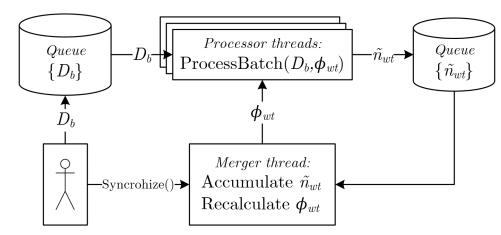
\includegraphics[natwidth=501bp,natheight=235bp,width=270bp]{old_arch.png}

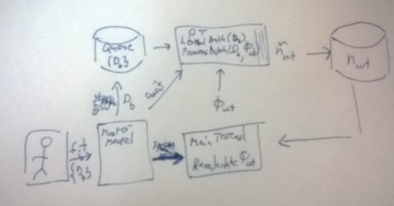
\includegraphics[natwidth=394bp,natheight=206bp,width=270bp]{new_arch.png}

\section{Experiments}
\label{sec:Experiments}

\section{Conclusions}
\label{sec:Conclusions}

TBD

\bigskip
\subsubsection*{Acknowledgements.}

TBD

%%%%%%%%%%%%%%%%%%%%%%%%%%%%%%%%%%%%%%%%%%%%%%%%%%%%%%%%%%%%%%%%%%%%%%%%%%%%
%\bibliographystyle{splncs03}
%\bibliography{MachLearn}

\begin{thebibliography}{10}
%\providecommand{\url}[1]{\texttt{#1}}
%\providecommand{\urlprefix}{URL }

TBD

\end{thebibliography}

\end{document}

